\chapter{Исследование LQR}
\label{ch:chap1}
\section{Условие задачи}

Рассмотреть систему:
$$
  \dot{x} = Ax + Bu, \tab x(0) = \begin{bmatrix} 1 & 1 & 1\end{bmatrix}^T
$$ и выполнить следующие шаги:

\begin{itemize}
\item Проверить систему на стабилизируемость.
\item Построить схему моделирования системы, замкнутой регулятором $u = Kx$.
\item Задаться подходящими значениями матриц $Q^∗ \succeq 0$ и $R^∗ \succ 0$ и 
значением параметра $\alpha > 0$ и сформировать четыре набора пар матриц $(Q,R)$:
\begin{itemize}
  \item $(Q,R);$
  \item $(\alpha Q,R);$
  \item $(Q, \alpha R);$
  \item $( \alpha Q, \alpha R);$
\end{itemize}
\item Для каждой из пар значений матриц $(Q,R)$ синтезировать регулятор, 
минимизирующий функционал качества путём решения матричного уравнения Риккати для $\nu = 1$:
\begin{itemize}
  \item  Найти соответствующую матрицу регулятора $K$, обеспечивающую миниминацию 
  функционала качества.
  \item Вычислить соответствующее минимизированное значение функционала качества 
  $$J_{min} = x_0^T P x_0$$
  \item Выполнить компьютерное моделирование замкнутой системы.
\end{itemize}
\item Сравнить полученные результаты для различных пар $(Q,R)$, сделать выводы.

\end{itemize}

\newpage
\section{Решение задачи}

Параметры для объекта:
$$
  A = \begin{bmatrix}
  12 & -1 & 14 \\
  6 & 0 & 6 \\
  -6 & -2 & -8 
  \end{bmatrix} \tab
  B = \begin{bmatrix}
    11 \\ 7 \\ -7 
  \end{bmatrix}
$$

Зададимся значениями матриц и параметра, на основе их сформируем четыре набора пар матриц $(Q,R)$:
$$
  \alpha = 20, \tab Q = \begin{bmatrix}
                        3 & 0 & 0 \\
                        0 & 3 & 0 \\
                        0 & 0 & 3 
                      \end{bmatrix}, \tab R=2
$$

\subsection{Исследование управляемости системы}

Найдём собственные числа матрицы $A$:
$$
    \lambda_{1,2} = 3 \pm 3i, \tab \lambda_3 = -2
$$

Воспользуемся результатами из прошлой работы. Система будет не полностью управляемой, но стабилизируемой, всю малину портит неуправляемое собственное число $\lambda_3 = -2$, но оно устойчивое.

\subsection{Первый набор}
$$
  Q = \begin{bmatrix}
                        3 & 0 & 0 \\
                        0 & 3 & 0 \\
                        0 & 0 & 3 
                      \end{bmatrix}, \tab R=2
$$

Синтезируем регулятор, минимизирующий функционал качества:
$$
  J = \int_{0}^{\infty} (x^T(t)Q x(t) + u^T(t) R u(t))dt  
$$
путем решения матричного уравнения Риккати при $\nu = 1$:
$$
    A^T P + PA + Q - \nu PBR^{-1}B^T P = 0, \tab K = -R^{-1}B^T P
$$
Положительно определённую матрицу $P$ мы сможем получить при выполнении следующих условий:
\begin{itemize}
  \item $Q \succeq 0$, $R \succ 0$
  \item $(A,B)$ - стабилизируемая пара
  \item $(Q, A)$ - наблюдаемая пара
\end{itemize}
Получим следующую матрицу регулятора $K$, обеспечивающую минимизацию функционала качества:
$$
   K = \begin{bmatrix} 10.42 & -10.13 &  10.12 \end{bmatrix}
$$

Получим следующее минимизированное значение функционала качества:
$$
   J_{min} = x_0^T P x_0 = \begin{bmatrix}
    1\\1\\1
   \end{bmatrix}^T \begin{bmatrix}
      
   48.61 &  -37.22 &  42.14 \\
  -37.22 &  29.40 & -31.98 \\
   42.14 & -31.98  & 37.13
   \end{bmatrix}
   \begin{bmatrix}
    1\\1\\1
   \end{bmatrix} = 61.02
$$

Выполним компьютерное моделирование замкнутой системы:

\begin{figure}[ht]
  \centering
  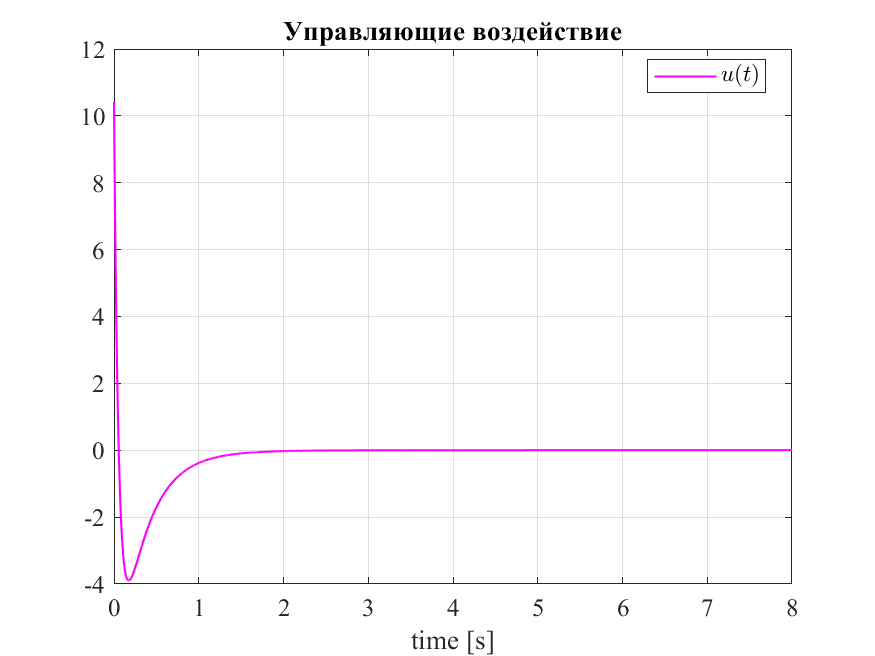
\includegraphics[width=0.8\textwidth]{lqr1_u1.png}
  \caption{Сигнал управления, LQR-регулятор $(Q, R)$}
\end{figure}
\newpage
\begin{figure}[ht]
  \centering
  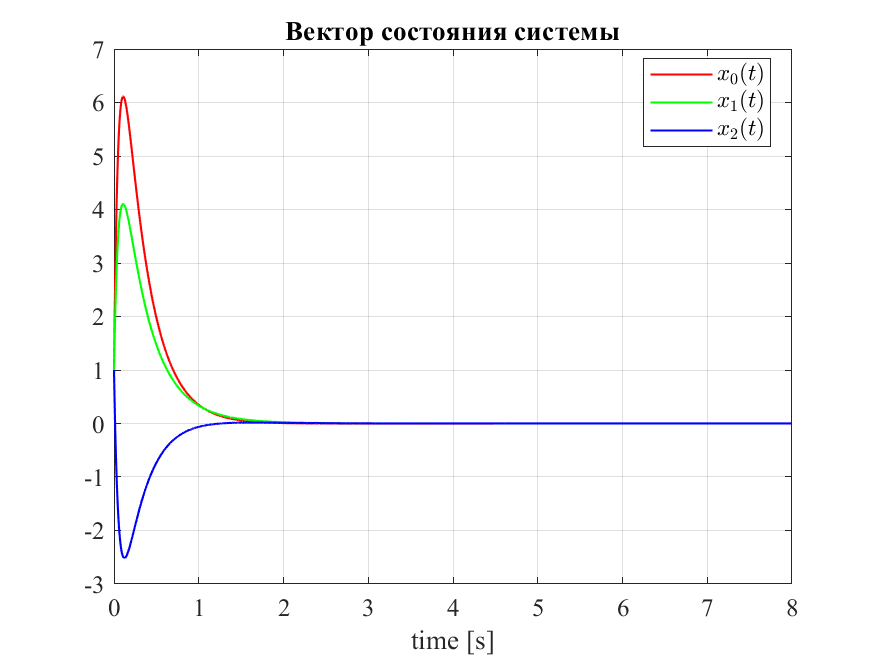
\includegraphics[width=0.8\textwidth]{lqr1_x1.png}
  \caption{Состояние системы, LQR-регулятор $(Q, R)$}
\end{figure}
\begin{figure}[ht]
  \centering
  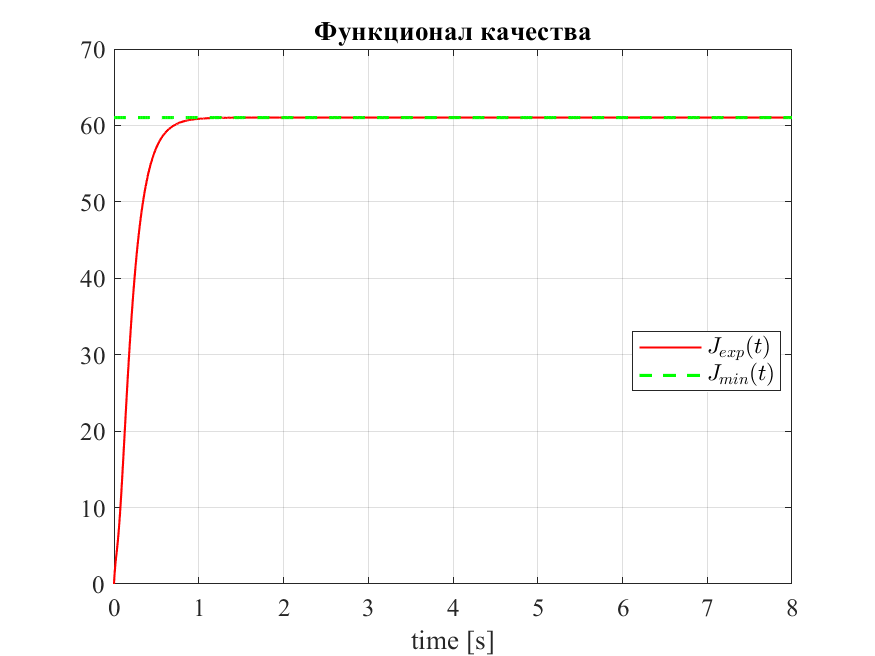
\includegraphics[width=0.8\textwidth]{funcJ1_1.png}
  \caption{Экспериментальное значение функционала качества, LQR-регулятор $(Q, R)$}
\end{figure}


\newpage
\subsection{Второй набор}
$$
  \alpha Q = \begin{bmatrix}
                        60 & 0 & 0 \\
                        0 & 60 & 0 \\
                        0 & 0 & 60 
                      \end{bmatrix}, \tab R=2
$$

По аналогии с первым пунктом, получим следующую матрицу регулятора $K$, обеспечивающую минимизацию функционала качества:
$$
   K = \begin{bmatrix} 22.24 & -20.51 &  21.12 \end{bmatrix}
$$

Получим следующее минимизированное значение функционала качества:
$$
   J_{min} = x_0^T P x_0 = 929
$$

Выполним компьютерное моделирование замкнутой системы:

\begin{figure}[ht]
  \centering
  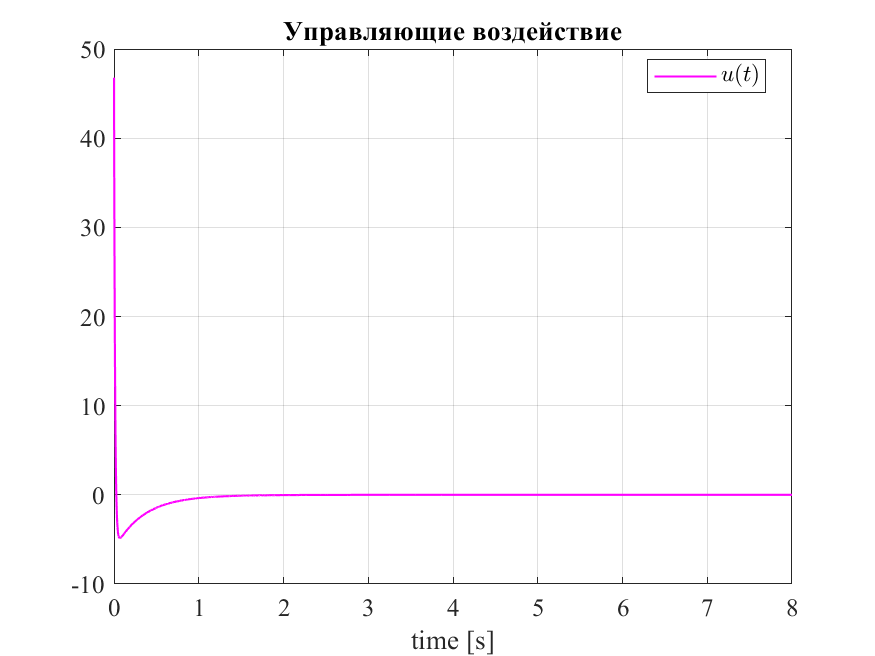
\includegraphics[width=0.8\textwidth]{lqr1_u2.png}
  \caption{Сигнал управления, LQR-регулятор $( \alpha Q, R)$}
\end{figure}
\newpage
\begin{figure}[ht]
  \centering
  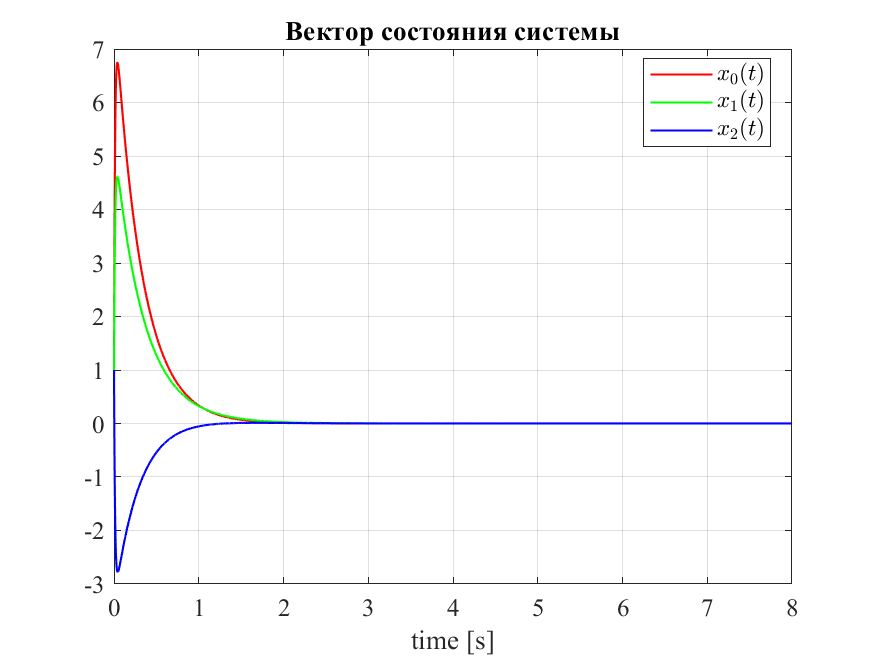
\includegraphics[width=0.8\textwidth]{lqr1_x2.png}
  \caption{Состояние системы, LQR-регулятор $(\alpha Q, R)$}
\end{figure}
\begin{figure}[ht]
  \centering
  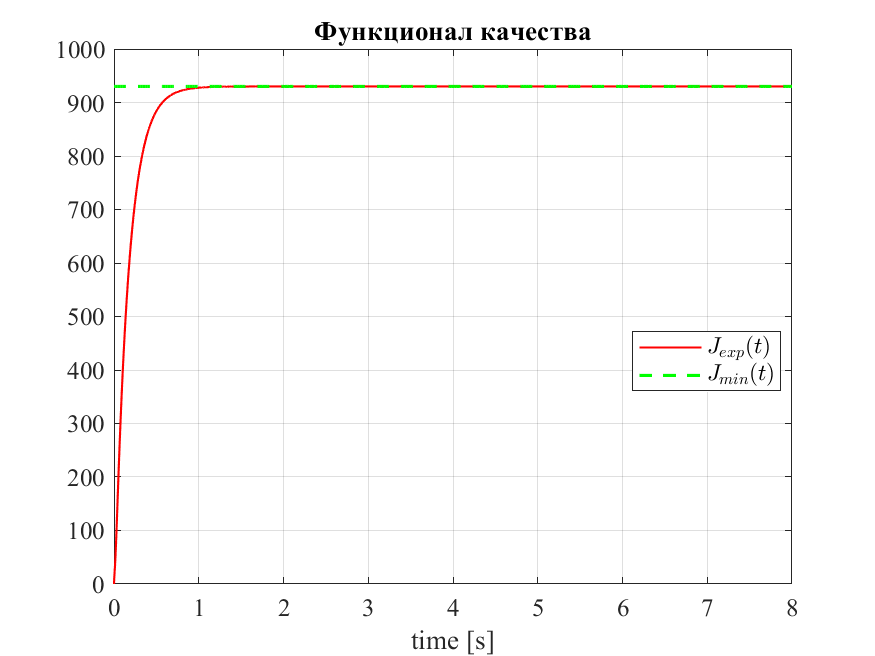
\includegraphics[width=0.8\textwidth]{funcJ1_2.png}
  \caption{Экспериментальное значение функционала качества, LQR-регулятор $(\alpha Q, R)$}
\end{figure}

\newpage
\subsection{Третий набор}
$$
  Q = \begin{bmatrix}
                        3 & 0 & 0 \\
                        0 & 3 & 0 \\
                        0 & 0 & 3 
                      \end{bmatrix}, \tab \alpha R=40
$$

По аналогии с первым пунктом, получим следующую матрицу регулятора $K$, обеспечивающую минимизацию функционала качества:
$$
   K = \begin{bmatrix} 5.39 & -5.66 &  5.28 \end{bmatrix}
$$

Получим следующее минимизированное значение функционала качества:
$$
   J_{min} = x_0^T P x_0 = 233
$$

Выполним компьютерное моделирование замкнутой системы:

\begin{figure}[ht]
  \centering
  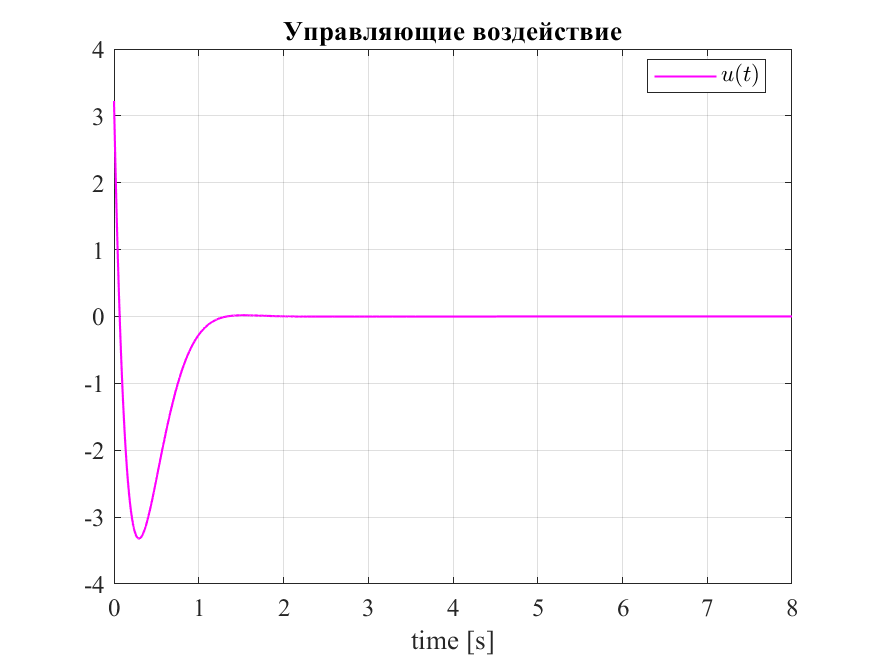
\includegraphics[width=0.8\textwidth]{lqr1_u3.png}
  \caption{Сигнал управления, LQR-регулятор $( \alpha Q, R)$}
\end{figure}
\newpage
\begin{figure}[ht]
  \centering
  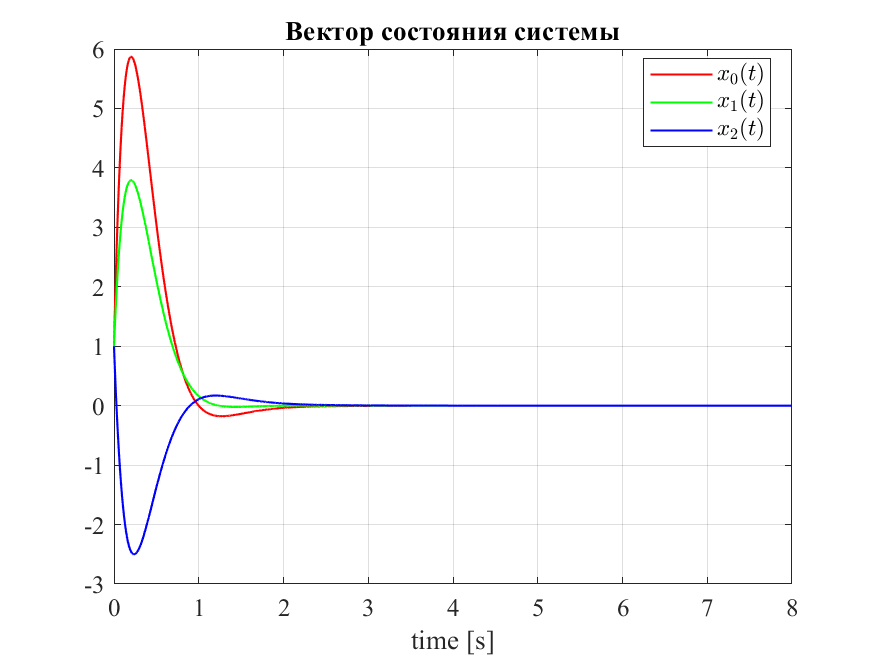
\includegraphics[width=0.8\textwidth]{lqr1_x3.png}
  \caption{Состояние системы, LQR-регулятор $(\alpha Q, R)$}
\end{figure}
\begin{figure}[ht]
  \centering
  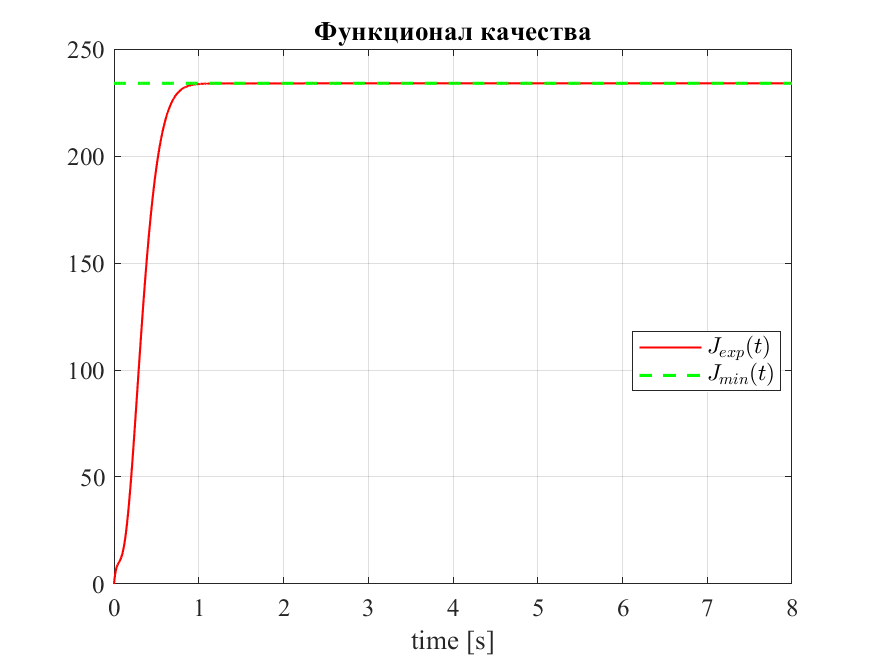
\includegraphics[width=0.8\textwidth]{funcJ1_3.png}
  \caption{Экспериментальное значение функционала качества, LQR-регулятор $(\alpha Q, R)$}
\end{figure}

\newpage
\subsection{Четвертый набор}
$$
  \alpha Q = \begin{bmatrix}
                      60 & 0 & 0 \\
                      0 & 60 & 0 \\
                      0 & 0 & 60 
                      \end{bmatrix}, \tab \alpha R=40
$$

По аналогии с первым пунктом, получим следующую матрицу регулятора $K$, обеспечивающую минимизацию функционала качества:
$$
   K = \begin{bmatrix} 10.42 & -10.13 &  10.12 \end{bmatrix}
$$

Получим следующее минимизированное значение функционала качества:
$$
   J_{min} = x_0^T P x_0 = 1220
$$

Выполним компьютерное моделирование замкнутой системы:

\begin{figure}[ht]
  \centering
  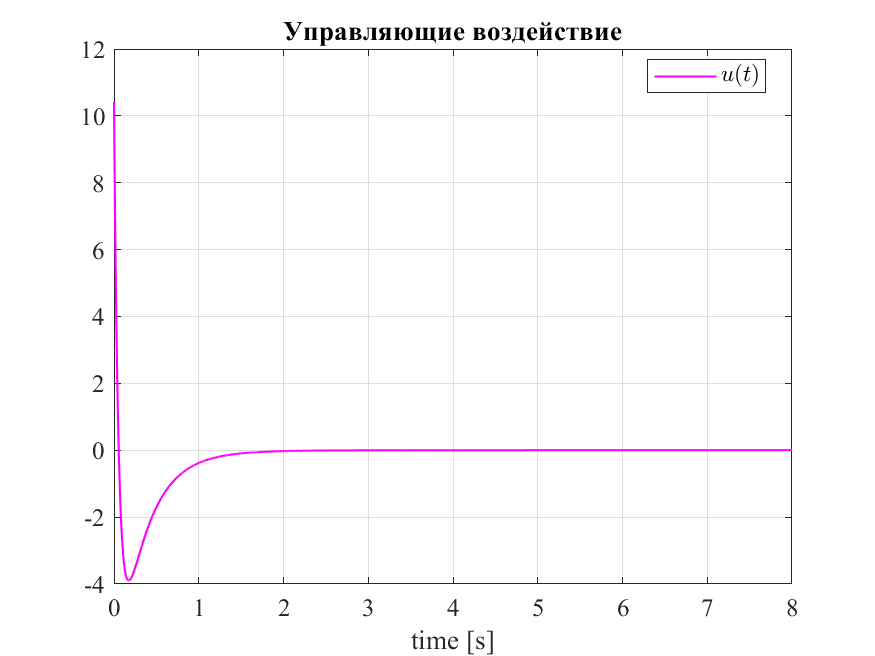
\includegraphics[width=0.8\textwidth]{lqr1_u4.png}
  \caption{Сигнал управления, LQR-регулятор $( \alpha Q, R)$}
\end{figure}
\newpage
\begin{figure}[ht]
  \centering
  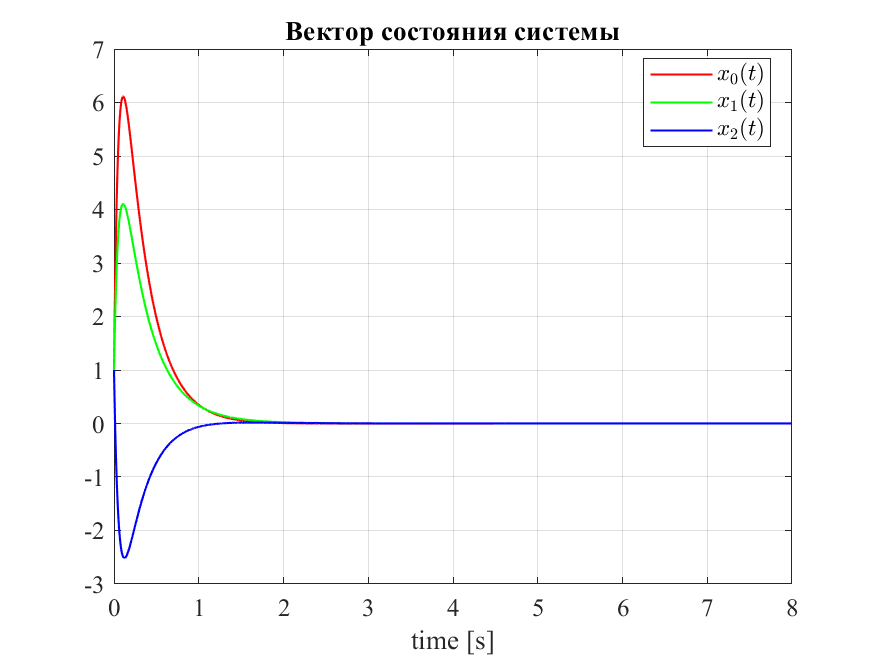
\includegraphics[width=0.8\textwidth]{lqr1_x4.png}
  \caption{Состояние системы, LQR-регулятор $(\alpha Q, R)$}
\end{figure}
\begin{figure}[ht]
  \centering
  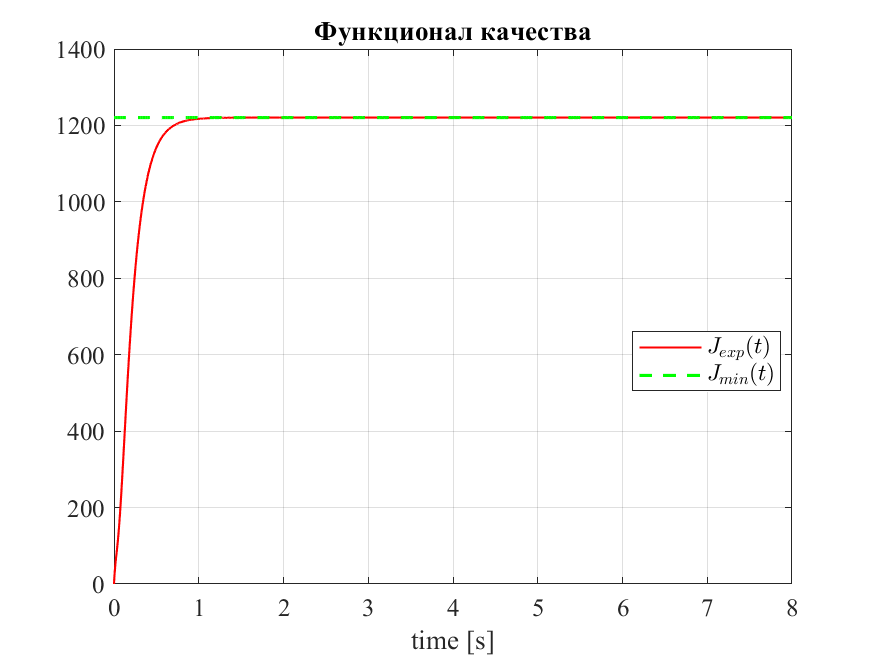
\includegraphics[width=0.8\textwidth]{funcJ1_4.png}
  \caption{Экспериментальное значение функционала качества, LQR-регулятор $(\alpha Q, R)$}
\end{figure}

\newpage
\subsection{Общее сравнение}

\begin{figure}[ht]
  \centering
  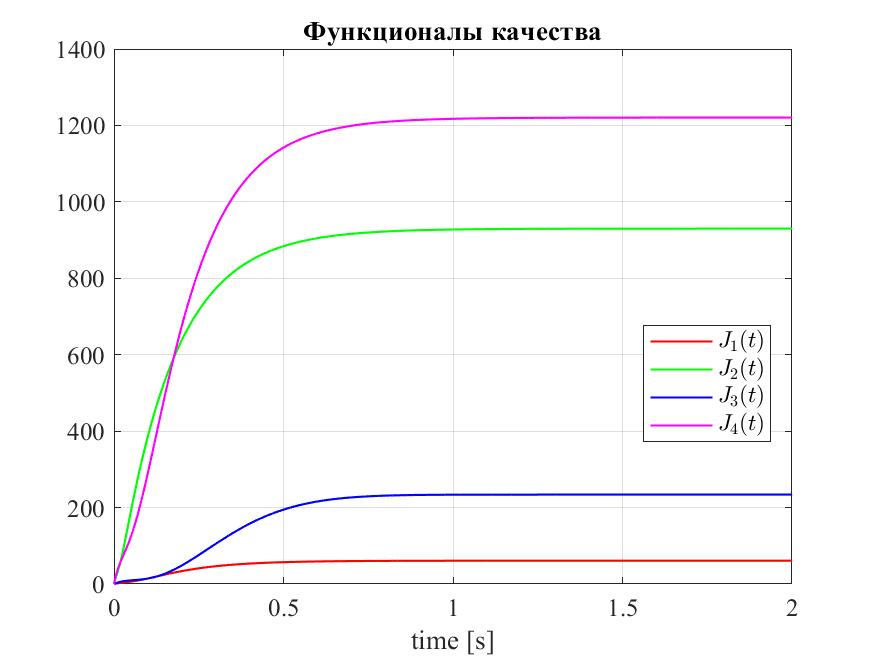
\includegraphics[width=0.8\textwidth]{funcJ1_all.png}
  \caption{Сравнение функционалов качества, LQR-регуляторы}
\end{figure}
\begin{figure}[ht]
  \centering
  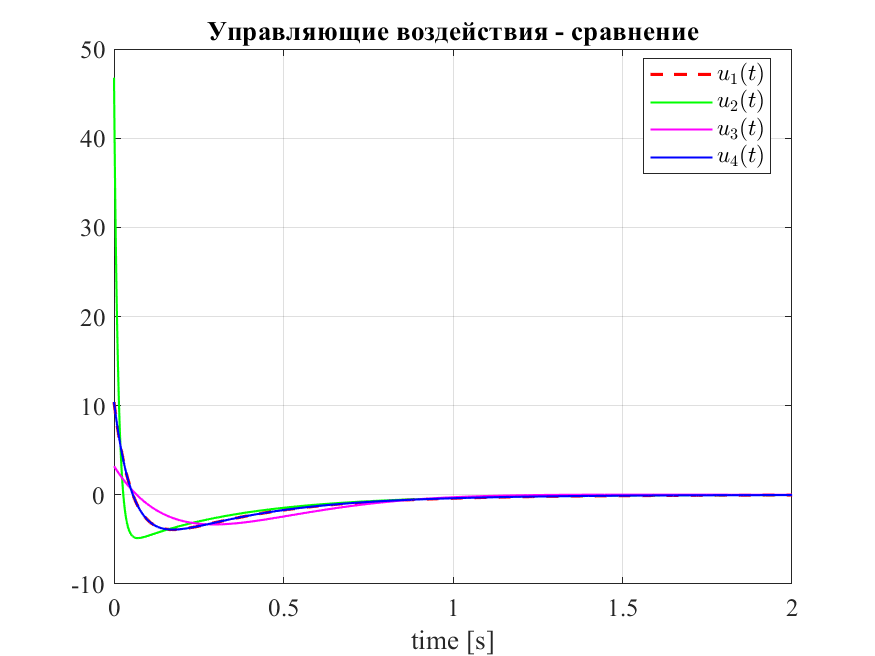
\includegraphics[width=0.8\textwidth]{lqr1_u_all.png}
  \caption{Сравнение управлений, LQR-регулятор}
\end{figure}

Можно заметить, что при бОльших требованиях к функционалу качества - когда мы требуем скорость побольше, или ставим штраф на управление больше, то в таких случаях он будет увеличиваться, что и прослеживается при обзоре.
В случае обзора графиков управления - при выставлении большого штрафа мы действительно уменьшаем управление по норме. Отдельного внимания заслуживает то, что коэффициенты регулятора совпали в 1-м и 4-м случае, 
хотя начальные параметры матриц отличаются на заметный коэффициент $\alpha$.

\subsection{Вывод}

В этом задании мы синтезировали LQR-регулятор, минимизировав функционал качества, который мы потребовали у регулятора. Данный регулятор является лучшим в смысле требований по критериям качества (скорость/затраты).
Регулятор отработал как и ожидалось.

\endinput